\documentclass[11pt,a4paper]{article}

% ---------------------------------------------------------------------------
% D-stability under first-order attachments at a single coordinate:
% an exact static threshold and a subset-sum criterion.
% Author metadata: set the three macros below before submission.
% ---------------------------------------------------------------------------
\newcommand{\PaperAuthor}{}
\newcommand{\PaperAffiliation}{}
\newcommand{\PaperDate}{September 2026}

\usepackage[T1]{fontenc}
\usepackage[utf8]{inputenc}
\usepackage{lmodern}
\usepackage{microtype}
\usepackage[a4paper,margin=1.05in]{geometry}
\usepackage{amsmath,amssymb,amsthm,mathtools}
\usepackage{booktabs}
\usepackage{array}
\usepackage{enumitem}
\usepackage{graphicx}
\usepackage{xcolor}
\usepackage{tikz}
\usetikzlibrary{arrows.meta,positioning,calc}
\usepackage[hyphens]{url}
\usepackage[colorlinks=true,linkcolor=blue!55!black,citecolor=blue!55!black,urlcolor=blue!55!black]{hyperref}
\hypersetup{pdftitle={D-stability under first-order attachments at a single coordinate: an exact static threshold and a subset-sum criterion},
  pdfauthor={\PaperAuthor},
  pdfsubject={D-stability, Hurwitz stability, robust stability, interconnected systems},
  pdfkeywords={D-stability, diagonal scaling, granularity, subset sums, value sets, negative-imaginary systems, buffers, decoys, Lean 4}}

\setlist{itemsep=2pt,topsep=3pt}
\setlength{\emergencystretch}{1.5em}

\theoremstyle{plain}
\newtheorem{theorem}{Theorem}[section]
\newtheorem{proposition}[theorem]{Proposition}
\newtheorem{lemma}[theorem]{Lemma}
\newtheorem{corollary}[theorem]{Corollary}
\newtheorem*{mainthm}{Main results}
\theoremstyle{definition}
\newtheorem{definition}[theorem]{Definition}
\newtheorem{example}[theorem]{Example}
\theoremstyle{remark}
\newtheorem{remark}[theorem]{Remark}

\newcommand{\R}{\mathbb{R}}
\newcommand{\C}{\mathbb{C}}
\newcommand{\Real}{\operatorname{Re}}
\newcommand{\Imag}{\operatorname{Im}}
\newcommand{\diag}{\operatorname{diag}}
\newcommand{\adj}{\operatorname{adj}}
\newcommand{\tr}{\operatorname{tr}}
\newcommand{\one}{\mathbf{1}}
\newcommand{\Env}{\Lambda}
\newcommand{\Core}{\Theta}
\newcommand{\Disk}{\mathbb{D}}

\title{D-stability under first-order attachments at a single coordinate:\\ an exact static threshold and a subset-sum criterion}
\author{\PaperAuthor\\[2pt]\small\PaperAffiliation}
\date{\PaperDate}

\begin{document}
\maketitle

\begin{abstract}
A real matrix is D-stable if it remains Hurwitz under every positive diagonal
rescaling, that is, for every choice of positive time scales of its
coordinates. We study a D-stable core that interacts with its environment
through a single coordinate, the port, to which a total load $G$ of
first-order attachments is coupled. Binding sites, decoys, buffers and
relaxing partner species are examples. The question is whether it matters how
the load is split into pieces with independent time scales. It does, and we
characterize exactly how. Let $\tau$ be the onset of instability along the static loading ray, the
infimum of the loads $X$ at which $B+Xe_pe_p^{T}$ is strictly D-unstable. Every partition of a total
$G<\tau$ is D-stable. At $G=\tau$ only a zero eigenvalue can occur. For
$G>\tau$ every sufficiently fine partition has a strictly growing mode at
finite, explicitly constructed rates. This threshold theorem is verified in
Lean~4. For a fixed partition, a closed-right-half-plane absorption identity
reduces D-stability to planar geometry: the core's
port response must stay below the lower envelope of semicircles erected over
the subset sums of the partition. Three
consequences follow. A partition is strictly unstable whenever one of its
subset sums lies in the static instability window. Merging pieces never
destroys D-stability. For an
explicit four-state family, the subset-sum test is exact throughout the
relevant range of loads. In that family a load of $2$ is safe for all time scales if and only
if a single piece carries at least $(7963+329\sqrt{409})/7780\approx1.8787$
of it: the split $(19/10,1/10)$ is D-stable, while $(15/8,1/8)$ and
$(1,1)$ are not. Four core states are necessary for such granularity
sensitivity. Bounding the ratio of time scales strictly raises the threshold
when $\det(B+\tau e_pe_p^{T})\ne0$. We extend the safety results to several
ports and to reciprocal relaxation modules, and we relate them to
negative-imaginary systems theory.
\end{abstract}

\noindent\textbf{Keywords:} D-stability; diagonal scaling; Hurwitz stability;
robust stability; value sets; subset sums; negative-imaginary systems;
buffers and decoys; formal verification.\\[2pt]
\textbf{MSC 2020:} 93D09, 15A18 (primary); 34D20, 93C05, 92C42 (secondary).

\tableofcontents

% =========================================================================
\section{Introduction}\label{sec:intro}

\paragraph{D-stability and unknown time scales.}
Let $\dot x=Bx$ be the linearization of a dynamical system at a steady state.
In many applications the entries of $B$ are known only up to the speed of each
variable: a species' compartment volume, turnover time or buffering capacity
rescales its row. Stability that survives every such choice is
\emph{D-stability}: $DB$ is Hurwitz for every positive diagonal matrix $D$.
The notion goes back to Enthoven and Arrow~\cite{enthoven1956} and Arrow and
McManus~\cite{arrow1958} in the stability of competitive equilibria. It has
since become a standard object in matrix theory, ecology and
biochemistry~\cite{johnson1974,cross1978,berman1983,hershkowitz1992,logofet1993,hornjohnson1991,kushel2019}.
Characterizing D-stability by finitely many algebraic conditions is classical
in dimension three~\cite{cain1976} and known in dimension
four~\cite{kanovei1998,impram2005}. In general it remains
open~\cite{kushel2019,kushel2026}. Related robust notions include strong
D-stability~\cite{abed1986} and structural stability of biochemical
networks~\cite{blanchini2014}. Recent work on chemical reaction networks
locates instability in small ``unstable cores''~\cite{vassena2024}.

\paragraph{The question.}
This paper does not attempt the general characterization. It asks a narrower
question, which arises whenever a stable subsystem is loaded through one of its
variables. Picture a \emph{core} $B$, for example a small gene or signalling
circuit, which is D-stable on its own. One of its variables, the \emph{port}
$p$, is shared with an environment of \emph{attachments}. Each attachment is
a single variable that is driven by the port, relaxes on its own time scale
and feeds back into the port (Figure~\ref{fig:schematic}). A reversible binding
site, a decoy, a buffer and a sequestering partner are all of this type. Every
attachment carries a \emph{load} $r_j>0$, which is the product of its forward
and return gains divided by its own damping; Section~\ref{sec:normalization}
makes this precise. The total load is $G=\sum_jr_j$. Now fix $G$. Is the
D-stability of the whole system determined by $G$ alone, or does it matter
whether the load arrives as one lump or as many fragments with independent
time scales?

\begin{figure}[t]
\centering
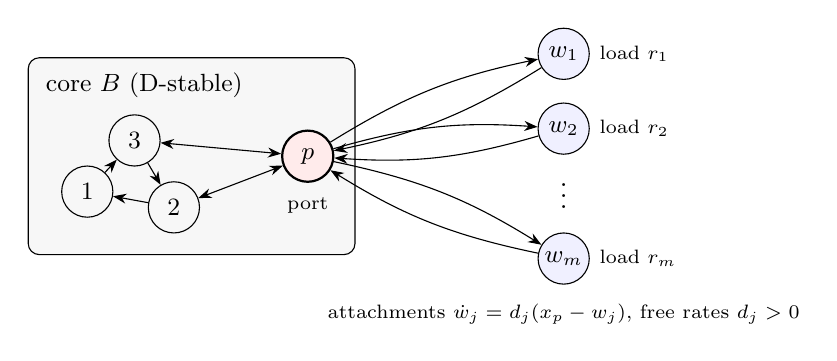
\begin{tikzpicture}[>=Stealth,node distance=6mm,
  st/.style={circle,draw,minimum size=6.5mm,inner sep=0pt,font=\small},
  lf/.style={circle,draw,fill=blue!6,minimum size=6.5mm,inner sep=0pt,font=\small}]
\draw[rounded corners,fill=gray!6] (-2.2,-1.25) rectangle (1.95,1.25);
\node[font=\small,anchor=north west] at (-2.1,1.18) {core $B$ (D-stable)};
\node[st] (c1) at (-1.45,-0.45) {$1$};
\node[st] (c2) at (-0.35,-0.65) {$2$};
\node[st] (c3) at (-0.85,0.2) {$3$};
\node[st,fill=red!8,thick] (p) at (1.35,0) {$p$};
\draw[->] (c1) -- (c3); \draw[->] (c3) -- (c2); \draw[->] (c2) -- (c1);
\draw[<->] (c2) -- (p); \draw[<->] (c3) -- (p);
\node[lf] (l1) at (4.6,1.3) {$w_1$};
\node[lf] (l2) at (4.6,0.35) {$w_2$};
\node at (4.6,-0.4) {$\vdots$};
\node[lf] (lm) at (4.6,-1.3) {$w_m$};
\foreach \l/\r in {l1/r_1,l2/r_2,lm/r_m}{
  \draw[->,bend left=10] (p) to (\l);
  \draw[->,bend left=10] (\l) to (p);
  \node[font=\scriptsize,anchor=west] at (\l.east) {load $\r$};}
\node[font=\scriptsize,align=center,anchor=north] at (4.6,-1.75) {attachments $\dot w_j=d_j(x_p-w_j)$, free rates $d_j>0$};
\node[font=\scriptsize,align=center] at (1.35,-0.62) {port};
\end{tikzpicture}
\caption{The interface architecture. A D-stable core interacts with $m$
first-order attachments only through one coordinate, the port $p$. Attachment
$j$ contributes load $r_j$ to the port equation. Every core and attachment
variable has its own unknown positive rate. The partition
$r=(r_1,\dots,r_m)$ of the total load $G$ is the object of study.}
\label{fig:schematic}
\end{figure}

\paragraph{The central mechanism.}
The answer turns on a simple observation. An attachment that is much faster
than the port behaves like an instantaneous extra term on the port's diagonal:
it shifts the port's self-coefficient by its load. An attachment that is much
slower than the port is effectively frozen and contributes nothing. An
attachment of intermediate speed contributes a phase lag. We show that this
lag can always be absorbed into the port's own free time scale
(Lemma~\ref{lem:absorb}). The dynamic problem therefore collapses onto the
\emph{static loading ray} $B_X=B+Xe_pe_p^{T}$, $0\le X\le G$. D-stability need
not be monotone along this ray: $B_X$ can be D-stable at both ends and strictly
D-unstable in a middle window. A single lump cannot produce an intermediate
effective load without also producing a large phase lag, and that lag protects
it (Section~\ref{sec:planar}). Fragments can instead be divided into a fast
group and a slow group. If a \emph{subset sum} of the pieces lies in the
unstable window, making that subset fast and the rest slow reproduces an
unstable static matrix (Figure~\ref{fig:window}).

\paragraph{Main results.}
Write $\tau$ for the onset of strict D-instability along the ray, the
infimum~\eqref{eq:tau} of the loads at which $B_X$ is strictly D-unstable.
\begin{enumerate}[label=(\Alph*),leftmargin=2.2em]
\item \emph{Exact threshold} (Theorem~\ref{thm:threshold}, verified in
Lean~4). Every positive partition of a total $G<\tau$ is D-stable. At $G=\tau$
the attached system is D-stable if and only if $\det B_\tau\ne0$. For
$G>\tau$ there is $\varepsilon>0$ such that every partition into pieces
smaller than $\varepsilon$ has a strictly unstable positive scaling. The
unstable eigenvalue of the static matrix is reproduced exactly, with rates
given in closed form (Lemma~\ref{lem:finite}).
\item \emph{Fixed partitions} (Theorem~\ref{thm:partition},
Corollary~\ref{cor:disk}). A fixed partition is D-stable if and only if a
determinant sign holds and the core's port response stays below the lower
envelope of an explicit family of semicircles over the subset sums. Equivalently, the response must lie in a
family of disks, a disk form reminiscent of the circle criterion. Consequences
(Section~\ref{sec:subsets}) are a subset-sum instability criterion, an exact
reduction of every verdict to one-attachment ``edges'' and static
``corners'', and monotonicity under merging.
\item \emph{An exactly solvable family} (Theorem~\ref{thm:family},
Corollary~\ref{cor:G2}). For an explicit rational four-state
family $B(h_0)$ the subset-sum criterion is exact, for any number of pieces and
every total $G\le h_0-4$. In particular, with
total load $2$ on the core $B(6)$, a partition is D-stable if and only if its
largest piece is at least $6-h_-=(7963+329\sqrt{409})/7780$. Four core
states are the minimum for any granularity effect
(Proposition~\ref{prop:small}).
\item \emph{Bounded time-scale heterogeneity} (Proposition~\ref{prop:spread}).
Above $\tau$, fine partitions are destabilized at a uniformly bounded ratio of
time scales. If $\det B_\tau\ne0$, any fixed bound on that ratio strictly
raises the effective threshold, so the required ratio diverges as
$G\downarrow\tau$.
\item \emph{Extensions} (Section~\ref{sec:extensions}). An open-box criterion
for several ports, safety for reciprocal relaxation modules, and a value-set
criterion for a hub joining several D-stable modules. The latter gives a
D-stability counterpart of the negative-imaginary stability theorem.
\end{enumerate}

\paragraph{Relation to previous work.}
Value sets and zero exclusion are the basic tools of parametric robust
control~\cite{barmish1994}. Our fixed-partition test is a value-set statement
in which the uncertain parameters are the time scales. The absorption identity
is what makes the value set of each attachment explicitly planar. The disk
form recalls the circle criterion~\cite{zames1966}, although the disks here
come from the partition rather than from a sector bound. Lanzon and
Petersen~\cite{lanzon2008,xiong2010,petersen2010} showed that a
negative-imaginary feedback loop is stable exactly when its DC loop gain is
suitably bounded. Our hub criterion (Theorem~\ref{thm:hub}) has the same
flavour when every module is negative imaginary for every scaling. The
attachment theorem, however, does not assume the core to be negative
imaginary: it retains the \emph{first} static loss along the ray instead of an
endpoint test. That is what allows a stable-to-unstable-to-stable pattern
along the loading ray. Reciprocal relaxation modules are classical relaxation
systems~\cite{willems1976,chaffey2023}. Fast and slow attachments are
singular-perturbation limits~\cite{kokotovic1999}. The robustness of loaded
systems to uncertain load time constants was studied for power
systems~\cite{nguyen2014}. In biology, buffers can create or suppress calcium
oscillations~\cite{falcke2003,gin2006}. Decoy binding sites and slow unbinding
shape biomolecular clocks~\cite{karapetyan2015,dey2021}. Loading of a module by
downstream binding, known as retroactivity, alters its
dynamics~\cite{delvecchio2008,jayanthi2013}. These phenomena are known, and we
do not claim them. Our contribution is an exact linear mechanism and
classification: which distributions of a fixed load can destabilize a fixed
linearized core for \emph{some} choice of time scales, and which cannot for
\emph{any}. We are not aware of a previous statement of the threshold theorem,
the subset-sum criterion or the four-state minimum.

\paragraph{Organization and evidence.}
Section~\ref{sec:setting} fixes conventions and derives the normalized model
from physical attachments. Sections~\ref{sec:absorb}--\ref{sec:threshold}
prove the threshold theorem. Sections~\ref{sec:planar}--\ref{sec:subsets}
treat fixed partitions. Section~\ref{sec:small} settles the minimum
dimension, and Section~\ref{sec:family} solves the four-state family.
Section~\ref{sec:extensions} contains the extensions,
Section~\ref{sec:application} the application to binding sites and buffers,
and Section~\ref{sec:verification} the verification status of every result.
Theorem~\ref{thm:threshold} is formally verified. Lemma~\ref{lem:edgecert}
is an exact computer-assisted certificate. All other proofs are
conventional and are given in full.

% =========================================================================
\section{Setting}\label{sec:setting}

\subsection{Conventions}
A real square matrix $M$ is \emph{Hurwitz} if all its eigenvalues satisfy
$\Real\lambda<0$. A \emph{positive scaling} of $M$ is $DM$ with
$D=\diag(d_1,\dots,d_N)$, $d_i>0$. Since $DM=D(MD)D^{-1}$, left and right
scalings have the same spectra; the Lean formalization uses right scalings.
We say that $M$ has \emph{strict growth}, or has a \emph{strictly unstable
positive scaling}, if some $DM$ has an eigenvalue with $\Real\lambda>0$. $M$
is \emph{D-stable} if every $DM$ is Hurwitz. D-stable matrices are
nonsingular, and marginal cases lie between the two notions: a matrix
without strict growth may still have a scaling with an imaginary-axis
eigenvalue, which we call a \emph{contact}.

It is often convenient to work with \emph{inverse rates} $Q=D^{-1}$: $\lambda$
is an eigenvalue of $DM$ exactly when the pencil $\lambda Q-M$ is singular.
Since $M$ is real, contacts $\pm i\omega$ come in conjugate pairs. Replacing
$Q$ by $\omega Q$ moves a contact at $i\omega$, $\omega>0$, to $i$. We use
this frequency normalization repeatedly; it is legitimate only because
\emph{all} rates are free.

\subsection{The attached system}
Fix a D-stable $n\times n$ matrix $B$, a coordinate $p$ with unit vector
$e=e_p$, and a finite \emph{partition} $r=(r_1,\dots,r_m)$ with every
$r_j>0$ and total $G=\sum_jr_j$. The attached matrix and the static loading
ray are
\begin{equation}\label{eq:attached}
 A_r=\begin{pmatrix}B&er^{T}\\ \one e^{T}&-I_m\end{pmatrix},\qquad
 B_X=B+X\,ee^{T}\quad(X\in\R).
\end{equation}
Attachment $j$ obeys $\dot w_j=d_{n+j}(x_p-w_j)$, and the port equation
receives $\sum_jr_jw_j$. All $n+m$ rates are free.

\subsection{From physical attachments to normalized loads}\label{sec:normalization}
A general scalar attachment has a port gain $a_j$ (the effect of $w_j$ on
$\dot x_p$), a capture gain $c_j$ (the effect of $x_p$ on $\dot w_j$) and a
damping $h_j>0$:
\[
 \dot w_j=d_j\,(c_jx_p-h_jw_j),\qquad \dot x_p=d_p\,\bigl((Bx)_p+a_jw_j\bigr).
\]
Three changes of variables bring this to \eqref{eq:attached}.
\begin{enumerate}[label=(\roman*)]
\item \emph{Absorb the damping into the rate.} Put $d_j'=d_jh_j$. Since $d_j$
is free, so is $d_j'$, and the attachment row becomes
$d_j'\bigl((c_j/h_j)x_p-w_j\bigr)$.
\item \emph{Rescale the state.} Assume $c_j\ne0$; otherwise the attachment
does not couple back. Put $w_j=(c_j/h_j)\tilde w_j$. This is a
diagonal similarity, and diagonal similarities commute with diagonal scalings,
so D-stability is unaffected. The attachment row becomes
$d_j'(x_p-\tilde w_j)$ and the port receives $r_j\tilde w_j$ with
\[
 r_j=\frac{a_jc_j}{h_j}.
\]
\item \emph{Signs.} The algebra in (ii) is valid for either sign of $c_j$, so
only the sign of the load $r_j$ matters. Positive loads,
$a_jc_j>0$, are positive-feedback partners, and they are the subject of this
paper. Negative loads are damping partners (Remark~\ref{rem:negative}).
\end{enumerate}
The dictionary for reversible binding sites and buffers is given in
Section~\ref{sec:application}. For such sites the load is
$r=ku/(u+\delta)$ for binding coefficient $k$, unbinding rate $u$ and
bound-complex degradation $\delta$, and the site also adds a loss $k$ to the
port diagonal.

\subsection{The static threshold}
The static loading ray is the family of matrices obtained by making every
attachment infinitely fast. Its first loss of stability is the quantity that
governs everything below:
\begin{equation}\label{eq:tau}
 \tau=\inf\{X\ge0:\ B_X\text{ has a strictly unstable positive scaling}\}.
\end{equation}

\begin{lemma}\label{lem:taubound}
$0\le\tau\le-B_{pp}$.
\end{lemma}
\begin{proof}
A D-stable matrix has nonpositive diagonal: if $B_{pp}>0$, scaling row $p$ by
$1$ and all other rows by $\eta\to0$ gives an eigenvalue near $B_{pp}>0$. If
$X>-B_{pp}$, the $(p,p)$ entry of $B_X$ is positive. Scaling row $p$ by a large
factor makes the trace positive, so some eigenvalue has positive real part.
Hence every $X>-B_{pp}$ belongs to the set in \eqref{eq:tau}.
\end{proof}

The set in \eqref{eq:tau} is open, because a strict eigenvalue persists under
small perturbations of $X$ at a fixed scaling. It does not contain $0$, because
$B$ is D-stable. Consequently, for every $X>\tau$ the interval $(\tau,X)$ contains a load with
strict growth, and if $\tau>0$ then $B_\tau$ has no strict growth.

% =========================================================================
\section{Absorption and static safety}\label{sec:absorb}

The following identity is the engine of the paper. It says that at any
candidate eigenvalue in the closed right half-plane, a first-order attachment
is indistinguishable from a static load \emph{smaller} than its own, plus an
increase of the port's inverse rate.

\begin{lemma}[Closed-half-plane absorption]\label{lem:absorb}
Let $z=\sigma+i\omega\ne0$ with $\sigma\ge0$, and let $r,t>0$. Put
\begin{equation}\label{eq:absorb}
 d=(1+\sigma t)^2+\omega^2t^2,\qquad \alpha=\frac{rt}{d},\qquad
 x=\frac{r(1+2\sigma t)}{d}.
\end{equation}
Then $\alpha>0$, $0<x<r$, and
\begin{equation}\label{eq:identity}
 \frac{r}{1+zt}+z\alpha=x .
\end{equation}
\end{lemma}
\begin{proof}
Here $d=|1+zt|^2>0$ and $r/(1+zt)=r(1+\bar zt)/d$. Adding $z\alpha=zrt/d$
gives $r(1+\bar zt+zt)/d=r(1+2\sigma t)/d=x$. Finally
$r-x=r(d-1-2\sigma t)/d=r|z|^2t^2/d>0$.
\end{proof}

Write the inverse rates of the attached system as $\hat Q=\diag(Q,t_1,\dots,
t_m)$, with $Q>0$ the core part. If $(\lambda\hat Q-A_r)(v,u)=0$ and
$1+\lambda t_j\ne0$, the attachment rows give $u_j=v_p/(1+\lambda t_j)$. The
core rows then give
\begin{equation}\label{eq:reduced}
 \Bigl(\lambda Q-B-L_r(\lambda)\,ee^{T}\Bigr)v=0,\qquad
 L_r(\lambda)=\sum_{j=1}^m\frac{r_j}{1+\lambda t_j}.
\end{equation}
Conversely, a nonzero solution $v$ of \eqref{eq:reduced} extends to an
eigenvector. Moreover, $v=0$ forces $u=0$, and
\[
 \det(\lambda\hat Q-A_r)=\prod_j(1+\lambda t_j)\cdot
 \det\bigl(\lambda Q-B-L_r(\lambda)ee^{T}\bigr).
\]
At $\lambda=0$, block elimination gives $\det(-A_r)=\det(-B_G)$.

\begin{theorem}[Static-interval safety]\label{thm:safety}
Suppose that $B_X$ is D-stable for every $0<X<G$. Then for every positive
partition $r$ of $G$ and every positive scaling, every nonzero eigenvalue of
the scaled $A_r$ has negative real part. Moreover $A_r$ is D-stable if and only
if $\det B_G\ne0$. If $\det B_G=0$, then $0$ is an eigenvalue of every positive
scaling of $A_r$.
\end{theorem}
\begin{proof}
Let $\lambda\ne0$ with $\Real\lambda\ge0$ be an eigenvalue at inverse rates
$\hat Q$. Then $1+\lambda t_j\ne0$, so \eqref{eq:reduced} holds with $v\ne0$.
Apply Lemma~\ref{lem:absorb} to every term of $L_r(\lambda)$:
$L_r(\lambda)=X-\lambda\sum_j\alpha_j$ with $X=\sum_jx_j\in(0,G)$ and
$\alpha_j>0$. Then \eqref{eq:reduced} reads
$(\lambda Q'-B_X)v=0$ with $Q'=Q+(\sum_j\alpha_j)ee^{T}$, again positive
diagonal. So $\lambda$ is a closed-right-half-plane eigenvalue of a positive
scaling of $B_X$, contradicting D-stability. Zero is an eigenvalue if and only
if $\det(-A_r)=\det(-B_G)$ vanishes, and this does not depend on the rates.
\end{proof}

The proof treats real and complex candidates alike. It needs neither
continuation along paths of rates nor any stability assumption on the
principal submatrix obtained by deleting the port. At $\sigma=0$, with the frequency normalized to $\omega=1$, it
specializes to the familiar phase absorption
$X=\sum_jr_j/(1+t_j^2)$, $q_p'=q_p+\sum_jr_jt_j/(1+t_j^2)$.

% =========================================================================
\section{The exact threshold}\label{sec:threshold}

\begin{lemma}[Static marginality below first strict growth]\label{lem:marginal}
$B_X$ is D-stable for every $0\le X<\tau$.
\end{lemma}
\begin{proof}
For $X<\tau$ there is no strict growth by definition, and $X=0$ is the
hypothesis. Suppose some $0<X<\tau$ has a contact: $\det(i\omega Q-B_X)=0$ for
some $Q>0$ and $\omega\in\R$. Put $P(z)=zQ-B$ and let
$c(z)=\adj(P(z))_{pp}$ be the $(p,p)$ cofactor. The cofactor does not depend on
the $(p,p)$ entry of $P$. Expansion along row $p$ gives
\[
 \det\bigl(P(z)-Yee^{T}\bigr)=\det P(z)-Y\,c(z)\qquad(Y\in\C).
\]
At the contact, $\det P(i\omega)\ne0$ because $B$ is D-stable, hence
$c(i\omega)\ne0$. The quotient $f=\det P/c$ is therefore analytic near
$i\omega$, with $f(i\omega)=X$. Changing the port inverse rate from $q_p$ to
$q_p+k$ replaces $P(z)$ by $P(z)+zk\,ee^{T}$ without changing $c$. So the
loaded, re-rated pencil is singular at $z$ exactly when
\begin{equation}\label{eq:perturb}
 f(z)+zk-Y=0 .
\end{equation}
Take $z=\sigma+i\omega$ with small $\sigma>0$. If $\omega\ne0$, solve
\eqref{eq:perturb} by $k(\sigma)=-\Imag f(z)/\omega$ and
$Y(\sigma)=\Real f(z)+\sigma k(\sigma)$. If $\omega=0$, take $k=0$ and
$Y=f(\sigma)$, which is real. In both cases $k(\sigma)\to0$ and
$Y(\sigma)\to X$ as $\sigma\downarrow0$, since $f(i\omega)=X$ is real. For
small $\sigma$ the inverse rate $q_p+k(\sigma)$ is positive and $Y(\sigma)>0$,
and $B_{Y(\sigma)}$ has the eigenvalue $z$ with $\Real z=\sigma>0$. Thus
$\tau\le Y(\sigma)$ for all small $\sigma$, so $\tau\le X$, a contradiction.
\end{proof}

The next lemma turns static growth into dynamic growth of every sufficiently
fine partition, preserving the unstable eigenvalue exactly.

\begin{lemma}[Finite realization of static growth]\label{lem:finite}
Let $0<X<G$, and suppose that $B_X$ has an eigenvalue $z=\sigma+i\omega$ with
$\sigma>0$ at inverse rates $Q>0$. Put $q=Q_{pp}$, $k=|z|^2$ and
$f(t)=(1+2\sigma t)/(1+2\sigma t+kt^2)$. Choose $\delta>0$ with
\begin{equation}\label{eq:quant}
 G\delta+\frac{Gk\delta^2}{2\sigma}\le\frac q2,\qquad Gk\delta^2<G-X,
\end{equation}
and put $\varepsilon=\min\{G-X,\;X(1-f(\delta))/2\}>0$. Then:
\begin{enumerate}[label=(\alph*)]
\item every partition of $G$ with $\max_jr_j<\varepsilon$ has a positive
scaling $D$ such that $z$ itself is an eigenvalue of $DA_r$;
\item the rates of (a) can be chosen in a compact subset of $(0,\infty)$ that
depends on $B,X,z,Q,G$ but not on the partition.
\end{enumerate}
\end{lemma}
\begin{proof}
The function $f$ decreases from $1$ to $0$ on $(0,\infty)$, since
$f'(t)=-2kt(1+\sigma t)/(1+2\sigma t+kt^2)^2$. Also
$1-f(\delta)=k\delta^2/(1+2\sigma\delta+k\delta^2)\in(0,k\delta^2]$.

Order the pieces arbitrarily and let $S$ be the first partial sum exceeding
$X$. Consecutive partial sums differ by less than $\varepsilon$, so
$X<S<X+\varepsilon\le G$; in particular some pieces remain after this group.
Give the pieces of this first group inverse rate $\delta$ (``fast''), and give
the remaining pieces a common inverse rate $T$ (``slow'') determined by
\begin{equation}\label{eq:T}
 f(T)=y:=\frac{X-Sf(\delta)}{G-S}.
\end{equation}
We check that $y\in(0,1)$ with bounds independent of the partition. First,
$Sf(\delta)<(X+\varepsilon)f(\delta)\le Xf(\delta)+\varepsilon$, so
$X-Sf(\delta)>X(1-f(\delta))-\varepsilon\ge X(1-f(\delta))/2$, and
$y\ge y_-:=X(1-f(\delta))/(2G)>0$. Second,
$G-S-(X-Sf(\delta))=G-X-S(1-f(\delta))\ge G-X-Gk\delta^2>0$, so
$1-y\ge(G-X-Gk\delta^2)/G$, that is, $y\le y_+<1$. Since $f$ is a decreasing
bijection $(0,\infty)\to(0,1)$, the solution
\[
 T=\frac{\sigma(1-y)+\sqrt{\sigma^2(1-y)^2+ky(1-y)}}{ky}
\]
exists, is unique, and lies in the compact interval $[f^{-1}(y_+),f^{-1}(y_-)]$.

With these inverse rates, the quantities $x_j$ of \eqref{eq:absorb} are
$x_j=r_jf(t_j)$. Hence $\sum_jx_j=Sf(\delta)+(G-S)y=X$. For the lag shifts,
each fast piece has $\alpha_j=r_j\delta/d_j\le r_j\delta$, so these sum to at
most $G\delta$. Each slow piece has $\alpha_j=x_jT/(1+2\sigma T)<x_j/(2\sigma)$,
and the slow $x_j$ sum to $X-Sf(\delta)<X(1-f(\delta))\le Gk\delta^2$. By
\eqref{eq:quant}, $\sum_j\alpha_j<q/2$.

Replace the port inverse rate $q$ by $q'=q-\sum_j\alpha_j\in(q/2,q)$ and keep the
other core inverse rates. By \eqref{eq:identity},
$L_r(z)=X-z\sum_j\alpha_j$, so
\[
 \Bigl(zQ'-B-L_r(z)ee^{T}\Bigr)v=\Bigl(zQ-B_X\Bigr)v=0
\]
for the static eigenvector $v$. By the remarks after \eqref{eq:reduced}, $z$ is
an eigenvalue of the scaled $A_r$. All
rates are fixed core rates, a port rate in $[1/q,2/q]$, $1/\delta$, or $1/T$ with $T$ in a fixed compact
interval.
\end{proof}

The constants in \eqref{eq:quant} are sufficient, not necessary. The
construction succeeds whenever $y\in(0,1)$ and $\sum_j\alpha_j<q$, and both
conditions can be checked directly for a given partition.

\begin{theorem}[Exact distribution-free granularity threshold]\label{thm:threshold}
Let $B$ be D-stable and let $\tau$ be defined by \eqref{eq:tau}. Then
$0\le\tau\le-B_{pp}$, and for every finite positive partition $r$ of $G$:
\begin{enumerate}[label=(\roman*)]
\item if $G<\tau$, then $A_r$ is D-stable;
\item if $G=\tau$, then $A_r$ is D-stable if and only if $\det B_\tau\ne0$.
Every nonzero eigenvalue of every positive scaling has negative real part, and
if $\det B_\tau=0$ then $0$ is an eigenvalue of every positive scaling;
\item if $G>\tau$, there is $\varepsilon>0$, independent of the number of
pieces, such that every partition of $G$ with all pieces smaller than
$\varepsilon$ has a strictly unstable positive scaling.
\end{enumerate}
\end{theorem}
\begin{proof}
The bounds are Lemma~\ref{lem:taubound}. If $G\le\tau$, then $B_X$ is D-stable
for $0<X<G$ by Lemma~\ref{lem:marginal}. For $G<\tau$, also $\det B_G\ne0$ by
the same lemma. Theorem~\ref{thm:safety} gives (i) and (ii). If $G>\tau$, the
infimum \eqref{eq:tau} provides $X\in[\tau,G)$ with strict growth, and $X>0$
because $B$ is D-stable. Lemma~\ref{lem:finite} gives (iii).
\end{proof}

\begin{remark}[What the theorem does and does not say]\label{rem:reduction}
Theorem~\ref{thm:threshold} is an exact \emph{reduction}. The dynamic question
about all partitions and all rates becomes a static D-stability question along
one ray. Evaluating $\tau$ is as hard as deciding D-stability of the matrices
$B_X$. It is explicit whenever that static problem can be solved: in dimensions
two and three (Section~\ref{sec:small}), in classified families
(Section~\ref{sec:family}), or from certificates. The theorem also says
nothing about \emph{coarse} partitions of $G>\tau$; those are the subject of
Sections~\ref{sec:planar}--\ref{sec:family}.
\end{remark}

\subsection{Bounded ratios of time scales}
In applications the time scales cannot be arbitrarily disparate. For a
positive diagonal $D$ let $\kappa(D)=\max_iD_{ii}/\min_iD_{ii}$ be its
\emph{spread}.

\begin{proposition}[Bounded spread raises the threshold]\label{prop:spread}
Let $B$ be D-stable.
\begin{enumerate}[label=(\alph*)]
\item For every $G>\tau$ there are $\varepsilon>0$ and $\kappa_G<\infty$ such that
every partition of $G$ into pieces smaller than $\varepsilon$ has a strictly
unstable scaling of spread at most $\kappa_G$.
\item Suppose $\det B_\tau\ne0$. For every $\kappa\ge1$ there is $\eta>0$ such
that for every $G<\tau+\eta$, every finite positive partition $r$ of $G$ and
every positive $D$ with $\kappa(D)\le\kappa$, the matrix $DA_r$ is Hurwitz.
\item If $\det(-B_G)<0$, then every positive scaling of every partition of $G$
has a positive real eigenvalue.
\end{enumerate}
Consequently, the time-scale-limited threshold
$\tau_\kappa=\sup\{G':\text{every partition of every }G<G'\text{ is Hurwitz at
all scalings of spread}\le\kappa\}$ is nonincreasing in $\kappa$ and tends to
$\tau$ as $\kappa\to\infty$. It satisfies $\tau_\kappa>\tau$ for every finite
$\kappa$ when $\det B_\tau\ne0$.
\end{proposition}
\begin{proof}
(a) is Lemma~\ref{lem:finite}(b) applied to one static witness $X\in(\tau,G)$.

(b) Suppose the claim fails for some $\kappa$. Then there are
$G_k\downarrow\tau$, partitions $r^{(k)}$ and scalings of spread at most
$\kappa$ with eigenvalues $\lambda_k$, $\Real\lambda_k\ge0$. By
Theorem~\ref{thm:threshold}, $G_k>\tau$. Multiplying a scaling by a
constant multiplies the spectrum by that constant, so we may normalize all
inverse rates to lie in $[1/\kappa,1]$. For $\Real\lambda\ge0$ and $t>0$ we
have $|1+\lambda t|\ge1$. Hence $|L_{r^{(k)}}(\lambda_k)|\le G_k$, and
\eqref{eq:reduced} with $\|v_k\|=1$ gives
$|\lambda_k|\le\kappa(\|B\|+G_k)$. Represent the attachments by the measures
$\mu_k=\sum_jr^{(k)}_j\delta_{t_j}$ on $[1/\kappa,1]$, of mass $G_k$, so that
$L_{r^{(k)}}(\lambda)=\int d\mu_k(t)/(1+\lambda t)$. Pass to a subsequence
along which $\mu_k\to\mu$ weakly, with mass $\tau$. Along it the core inverse
rates converge to $Q_*\in[1/\kappa,1]^n$, $\lambda_k\to\lambda_*$ with
$\Real\lambda_*\ge0$, and $v_k\to v_*$ with $\|v_*\|=1$. The integrands are
uniformly Lipschitz in $\lambda$ on $\{\Real\lambda\ge0\}$, so
$L_{r^{(k)}}(\lambda_k)\to L(\lambda_*)=\int d\mu/(1+\lambda_*t)$. In the limit,
\[
 \bigl(\lambda_*Q_*-B-L(\lambda_*)ee^{T}\bigr)v_*=0 .
\]
If $\lambda_*=0$, then $L(0)=\tau$ and $B_\tau v_*=0$, contradicting
$\det B_\tau\ne0$. If $\lambda_*\ne0$, integrate Lemma~\ref{lem:absorb}
against $\mu$: $L(\lambda_*)=x-\lambda_*\alpha$ with $\alpha\ge0$ and
$0\le x\le\tau$. If $\mu\ne0$ then $x<\tau$, because the integrand of $\tau-x$ is
positive on $[1/\kappa,1]$; if $\mu=0$ then $x=0$. In both cases $B_x$ is
D-stable, by Lemma~\ref{lem:marginal} or because $B_0=B$. Yet $\lambda_*$ is a
closed-right-half-plane eigenvalue of the positive scaling
$(Q_*+\alpha ee^{T})^{-1}B_x$. This is a contradiction.

(c) The characteristic polynomial of $DA_r$ is monic, and its constant term is
$\det(-DA_r)=\det D\cdot\det(-B_G)<0$. Hence it has a positive real root.

The consequences follow from (a), (b) and monotonicity in $\kappa$.
\end{proof}

Part (b) says that near a threshold with $\det B_\tau\ne0$, instability is
bought only with ever larger ratios of time scales. Part (c) says that a
real-root crossing, where $\det(-B_X)$ changes sign at $\tau$, is not softened
at all. For the four-state example of Section~\ref{sec:family}, an explicit
witness destabilizes the split $(1,1)$ with spread $4375/4$.

% =========================================================================
\section{Fixed partitions: planar geometry}\label{sec:planar}

Theorem~\ref{thm:threshold} classifies all sufficiently fine partitions. We now
decide a \emph{given} partition. Order the coordinates so that the port comes
first and write
\[
 B=\begin{pmatrix}b&a^{T}\\ c&C\end{pmatrix},\qquad
 Z(Q_c)=a^{T}(iQ_c-C)^{-1}c\quad(\det(iQ_c-C)\ne0),
\]
where $Q_c$ ranges over positive diagonal inverse rates of the $n-1$ inner
coordinates. We assume $n\ge2$. The \emph{core envelope} is
\begin{equation}\label{eq:coreenv}
 \Core(X)=\sup\bigl\{\Imag Z(Q_c):\ Q_c>0,\ \det(iQ_c-C)\ne0,\ \Real Z(Q_c)=-b-X\bigr\},
 \qquad \sup\varnothing=-\infty .
\end{equation}
Thus $\Core(X)>0$ means that the static matrix $B_X$ has a contact at some
scaling.

\subsection{The image of a partition}
At frequency one, the attachments contribute
$L_r(i)=\sum_jr_j/(1+it_j)=X-iY$. For $0<X<G$ define the \emph{protection
envelope}
\begin{equation}\label{eq:envelope}
 \Env_r(X)=\min_{(k,S)}\sqrt{(X-r(S))(r(S)+r_k-X)},
\end{equation}
the minimum being over all $1\le k\le m$ and $S\subseteq[m]\setminus\{k\}$ with
$r(S)\le X\le r(S)+r_k$,
where $r(S)=\sum_{j\in S}r_j$. The graph of $\Env_r$ is the lower envelope of
the semicircles with diameters $[r(S),r(S)+r_k]$. It vanishes exactly at the
subset sums of $r$. For one piece, $\Env_{(G)}(X)=\sqrt{X(G-X)}$.

\begin{lemma}[Exact attachment image]\label{lem:image}
As the inverse rates $t_j$ range over $(0,\infty)$, the point
$(X,Y)$ with $X-iY=\sum_jr_j/(1+it_j)$ ranges over
\begin{align*}
 &\{(X,\sqrt{X(G-X)}):\ 0<X<G\}&&\text{if }m=1,\\
 &\{(X,Y):\ 0<X<G,\ \Env_r(X)<Y\le\sqrt{X(G-X)}\}&&\text{if }m\ge2.
\end{align*}
\end{lemma}
\begin{proof}
One piece gives $x=r/(1+t^2)$ and $y=rt/(1+t^2)=\sqrt{x(r-x)}$. As $t$ ranges
over $(0,\infty)$, $x$ ranges over $(0,r)$ bijectively, with inverse
$t=\sqrt{(r-x)/x}$. Hence the attainable points are the images of
$\varphi(x)=\sum_j\sqrt{x_j(r_j-x_j)}$ on the open slices
$\Sigma_X^\circ=\{x\in\prod_j(0,r_j):\sum_jx_j=X\}$, $0<X<G$. By
Cauchy--Schwarz, $\varphi(x)\le\sqrt{\sum_jx_j}\sqrt{\sum_j(r_j-x_j)}
=\sqrt{X(G-X)}$, with equality at $x_j=r_jX/G$, which lies in
$\Sigma_X^\circ$. The function $\varphi$ is strictly concave on the closed
slice $\Sigma_X$, which is a polytope. Hence its minimizers over $\Sigma_X$ are
vertices. At a vertex at most one coordinate $x_k$ is strictly between its
bounds; the others equal $r_j$ ($j\in S$) or $0$. The vertex values are the
numbers in \eqref{eq:envelope}, so $\min_{\Sigma_X}\varphi=\Env_r(X)$. If
$m\ge2$, every vertex has a coordinate at a bound, so vertices are not in
$\Sigma_X^\circ$ and $\varphi>\Env_r(X)$ there. The image of the convex set
$\Sigma_X^\circ$ under the continuous $\varphi$ is an interval. Its infimum is
$\Env_r(X)$, because $\Sigma_X^\circ$ is dense in $\Sigma_X$, and its maximum
$\sqrt{X(G-X)}$ is attained.
\end{proof}

\subsection{The fixed-partition test}

\begin{theorem}[Exact fixed-partition test]\label{thm:partition}
Let $B$ be D-stable with $n\ge2$. Then $A_r$ is D-stable if and only if
\begin{equation}\label{eq:partitiontest}
 \det(-B_G)>0\qquad\text{and}\qquad \Core(X)\le\Env_r(X)\quad\text{for all }0<X<G.
\end{equation}
\end{theorem}
\begin{proof}
\emph{Zero eigenvalues.} $\det(-DA_r)=\det D\,\det(-B_G)$. A Hurwitz matrix
$M$ has $\det(-M)>0$, so the determinant condition is necessary. It excludes
zero eigenvalues.

\emph{Contacts.} After frequency normalization, a contact is a singular pencil
$i\hat Q-A_r$. Since $1+it_j\ne0$, this means
$\det(iQ-B-L_r(i)ee^{T})=0$ with $Q=\diag(q_h,Q_c)$. Suppose first
$\det(iQ_c-C)\ne0$. The Schur complement on the port gives
\[
 \det\bigl(iQ-B-L\,ee^{T}\bigr)=\det(iQ_c-C)\,\bigl(iq_h-b-L-Z(Q_c)\bigr).
\]
With $L=X-iY$, singularity means $X=-b-\Real Z$ and $q_h=\Imag Z-Y$. Given $Q_c$,
some positive $q_h$ and some attachment rates realize this if and only if
$X\in(0,G)$ and some attainable height $Y$ at $X$ satisfies $Y<\Imag Z$. By
Lemma~\ref{lem:image}, this happens if and only if $\Imag Z>\Env_r(X)$: for
$m\ge2$ the attainable heights are exactly $(\Env_r(X),\sqrt{X(G-X)}]$, and
for $m=1$ the only height is $\Env_{(G)}(X)$. Taking the supremum over $Q_c$,
contacts with a regular inner pencil exist if and only if
$\Core(X)>\Env_r(X)$ for some $X\in(0,G)$.

Singular inner pencils give no contacts. If $\det(iQ_c-C)=0$, expansion along
the port gives $\det(iQ-B-Lee^{T})=-a^{T}\adj(iQ_c-C)\,c$, independent of $L$
and $q_h$. With $L=0$ this is $\det(iQ-B)\ne0$, because $B$ is D-stable.

\emph{A stable base point.} Fix any positive core rates $D_c$ and give every
attachment rate $\epsilon$. At $\epsilon=0$ the scaled matrix is block
triangular with eigenvalues those of $D_cB$, which lie in the open left
half-plane, and $0$ with multiplicity $m$. For small $\epsilon>0$, $m$
eigenvalues lie in a small disk around $0$. The value $-\epsilon$ is an
eigenvalue of multiplicity at least $m-1$, with eigenvectors $x=0$,
$\sum_jr_jw_j=0$. The remaining eigenvalue $\lambda_s$ in the disk is real,
since its conjugate is also in the disk. Comparing determinants,
\[
 \lambda_s(-\epsilon)^{m-1}\prod(\text{fast eigenvalues})
 =\det(DA_r)=\epsilon^m\det D_c\,(-1)^m\det B_G,
\]
and the product of the fast eigenvalues tends to $\det(D_cB)$. Hence
\[
 \lambda_s=-\epsilon\,\frac{\det(-B_G)}{\det(-B)}\,\bigl(1+o(1)\bigr)<0,
\]
and the scaled matrix is Hurwitz for small $\epsilon$.

\emph{Conclusion.} If \eqref{eq:partitiontest} holds, no eigenvalue of any
positive scaling lies on the imaginary axis. The positive diagonal cone is
connected and eigenvalues depend continuously on the rates. Starting from the
Hurwitz base point, no eigenvalue can reach the closed right half-plane.
Conversely, D-stability excludes contacts and forces the determinant sign.
\end{proof}

The base-point computation also shows the role of the determinant condition:
when $\det(-B_G)<0$, the slow eigenvalue is positive.

\begin{corollary}[Disk form]\label{cor:disk}
For $1\le k\le m$ and $S\subseteq[m]\setminus\{k\}$ let $\Disk_{k,S}$ be the
closed disk in $\C$ with diameter $[-b-r(S)-r_k,\,-b-r(S)]$ on the real axis.
Then $A_r$ is D-stable if and only if $\det(-B_G)>0$ and every core value
$Z=Z(Q_c)$ with $\Imag Z>0$ and $-b-G<\Real Z<-b$ lies in every disk
$\Disk_{k,S}$ whose diameter contains $\Real Z$. For a single piece this is one
disk, with diameter $[-b-G,-b]$.
\end{corollary}
\begin{proof}
With $X=-b-\Real Z$ and $s=r(S)$, the inequality
$(\Imag Z)^2\le(X-s)(s+r_k-X)$ is
$(\Real Z+b+s+r_k/2)^2+(\Imag Z)^2\le(r_k/2)^2$. The condition
$\Imag Z\le\Env_r(X)$ requires this for every $(k,S)$ with
$s\le X\le s+r_k$.
\end{proof}

In the $Z$-plane, a lump offers one large disk. A fragmented load replaces it
by a chain of small disks that touch the real axis at every subset sum. Near a
subset sum no core value with positive imaginary part is tolerated.
Figure~\ref{fig:envelopes} shows the same picture in the coordinates
$(X,\Imag Z)$, where disks become semicircles.

\begin{remark}[Negative loads]\label{rem:negative}
For negative loads $r_j<0$ with total $G<0$, both $X$ and $Y$ in
$L_r(i)=X-iY$ are negative. A contact requires $q_h=\Imag Z-Y=\Imag Z+|Y|>0$.
Now the \emph{largest} attainable $|Y|$ at fixed $X$ is what matters. By the
Cauchy--Schwarz step of Lemma~\ref{lem:image} it equals $\sqrt{|X|(|G|-|X|)}$
and is attained with synchronized times. It depends on the total only. The
proof of Theorem~\ref{thm:partition} therefore shows that, for damping
partners, D-stability is independent of the partition. Granularity is a
positive-feedback phenomenon: for positive loads the protective height is the
\emph{minimum} over the partition's semicircles.
\end{remark}

% =========================================================================
\section{Subset sums, edges and corners}\label{sec:subsets}

The planar test has three practical consequences. The first reduces every
fixed-partition verdict to one-attachment systems and static matrices.

\begin{lemma}[Edges and corners]\label{lem:edges}
Let $B$ be D-stable and let $r$ be a partition of $G$. Suppose that
\begin{enumerate}[label=(\roman*)]
\item $\det(-B_G)>0$;
\item for every subset $S$ with $0<r(S)<G$, the static \emph{corner}
$B_{r(S)}$ is D-stable;
\item for every $k$ and $S\subseteq[m]\setminus\{k\}$, the one-attachment
\emph{edge} system, with core $B_{r(S)}$ and a single piece of load $r_k$, is
D-stable.
\end{enumerate}
Then $A_r$ is D-stable. Conversely, if $A_r$ is D-stable then (i)--(iii)
hold. There are at most $m2^{m-1}$ edges and $2^m$ corners; equal pieces
reduce these counts.
\end{lemma}
\begin{proof}
Suppose $\Core(X)>\Env_r(X)$ for some $X\in(0,G)$. Then some core value $Z$
has $\Real Z=-b-X$ and $\Imag Z>\Env_r(X)$. Choose $(k,S)$ attaining the
minimum in \eqref{eq:envelope}, and put $s=r(S)$. The core $B_s$ has the same
inner block and port self-coefficient $b+s$, so it has the same core values
$Z$. If $s<X<s+r_k$, then $X'=X-s\in(0,r_k)$ satisfies
$\Real Z=-(b+s)-X'$ and $\Imag Z>\sqrt{X'(r_k-X')}$. By
Theorem~\ref{thm:partition} applied to the edge, the edge has a contact,
contradicting (iii). If $X$ is an endpoint, then $X=s'$ is a subset sum in
$(0,G)$ and $\Env_r(X)=0<\Imag Z$. The static matrix $B_{s'}$ then has a
contact with port inverse rate $q_h=\Imag Z$, contradicting
(ii). Hence \eqref{eq:partitiontest} holds.

For the converse, let $A_r$ be D-stable. Then (i) holds by
Theorem~\ref{thm:partition}. The function $X\mapsto\det(-B_X)$ is affine and
positive at $X=0$ and $X=G$, hence positive on $[0,G]$. Let $s'$ be a subset sum
in $(0,G)$. By Proposition~\ref{prop:subsetsum}, $B_{s'}$ has no strict growth.
Since $\Core(s')\le\Env_r(s')=0$, no core value with $\Real Z=-b-s'$ has
positive imaginary part, so $B_{s'}$ has no contact through a regular inner
pencil. Singular inner pencils give none either (proof of
Theorem~\ref{thm:partition}). Together with $\det(-B_{s'})>0$, this makes the
corner $B_{s'}$ D-stable, proving (ii). For an edge $(k,S)$ with $s=r(S)$, the
core $B_s$ is D-stable (it is $B$ or a corner), its determinant condition is
$\det(-B_{s+r_k})>0$, and its core envelope at $X'\in(0,r_k)$ is
$\Core(s+X')\le\Env_r(s+X')\le\sqrt{X'(r_k-X')}$. Theorem~\ref{thm:partition}
applied to the edge gives (iii).
\end{proof}

The second consequence identifies the mechanism: fast pieces act as static
load and slow pieces vanish.

\begin{proposition}[Subset-sum obstruction]\label{prop:subsetsum}
Let $B$ be any real matrix and $r$ a partition. If for some
$S\subseteq[m]$ the static matrix $B_{r(S)}$ has a strictly unstable positive
scaling, then $A_r$ has a strictly unstable positive scaling. This holds in
particular for $S=\varnothing$ ($B$ itself) and for $S=[m]$ ($B_G$).
\end{proposition}
\begin{proof}
Let $B_{r(S)}$ have eigenvalue $z_0$ with $\Real z_0=\sigma_0>0$ at inverse
rates $Q$. Give the pieces in $S$ inverse rate $\epsilon$ and the others
inverse rate $1/\epsilon$. On the disk $K=\{|z-z_0|\le\rho\}$ with
$\rho<\sigma_0/2$ we have $\Real z\ge\sigma_0/2$. Using $|1+zt|\ge1$ and
$|1+z/\epsilon|\ge1+\sigma_0/(2\epsilon)$,
\[
 \Bigl|L_\epsilon(z)-r(S)\Bigr|\le\sum_{j\in S}\frac{r_j|z|\epsilon}{|1+z\epsilon|}
 +\sum_{j\notin S}\frac{r_j}{|1+z/\epsilon|}\le
 G\Bigl(|z|\epsilon+\frac{2\epsilon}{\sigma_0}\Bigr),
\]
uniformly on $K$. Hence $F_\epsilon(z)=\det(zQ-B-L_\epsilon(z)ee^{T})$
converges uniformly on $K$ to $F_0(z)=\det(zQ-B_{r(S)})$. Choose $\rho$ so that
$F_0$ has no zero on $\partial K$; $F_0$ is a nonzero polynomial. By
Hurwitz's theorem~\cite{conway1978}, $F_\epsilon$ has a zero in $K$ for small
$\epsilon$. By \eqref{eq:reduced} it is an eigenvalue of the scaled $A_r$ with
positive real part.
\end{proof}

The third consequence is monotonicity. A partition $r'$ \emph{refines} $r$ if
the pieces of $r'$ can be grouped so that the group sums are the pieces of $r$.

\begin{corollary}[Merging is safe]\label{cor:merge}
If $r'$ refines $r$, then every eigenvalue of a positive scaling of $A_r$ is an
eigenvalue of a positive scaling of $A_{r'}$. In particular, D-stability of
$A_{r'}$ implies D-stability of $A_r$, and a strictly unstable scaling of $A_r$
yields one for $A_{r'}$. The single lump $(G)$ is the most protective
partition: if any partition of $G$ is D-stable, so is $A_{(G)}$.
\end{corollary}
\begin{proof}
Give the pieces of $r'$ in each group the rate of the corresponding piece of
$r$. Then $L_{r'}=L_r$, and the characteristic polynomials satisfy
$\chi_{A_{r'}}=\chi_{A_r}\prod(s+d_\ell)^{\nu_\ell-1}$. Here group $\ell$ has
$\nu_\ell$ pieces and rate $d_\ell$, and the extra factors are the difference
modes inside the groups, all with eigenvalue $-d_\ell<0$. For the last
statement, note that $(G)$ is refined by every partition.
\end{proof}

Taken together, Theorem~\ref{thm:threshold}, Proposition~\ref{prop:subsetsum}
and Corollary~\ref{cor:merge} describe the landscape at a fixed total. The lump
is safest; merging pieces helps. A partition is doomed as soon as a subset sum
enters the static instability window. In the limit of fine dust, subset sums
are dense and only $\tau$ matters. Whether the subset-sum criterion is also
\emph{sufficient} depends on the core. By Lemma~\ref{lem:edges} it is
sufficient whenever, for the partitions in question, all corners are D-stable
as soon as they have no strict growth, and every edge is D-stable as soon as
its two static corners are.
Section~\ref{sec:family} gives a family where this holds.

% =========================================================================
\section{Small cores and the minimum dimension}\label{sec:small}

A granularity effect at fixed total requires the static ray to lose and then
regain stability. We show that this cannot happen in dimension at most three.

\paragraph{Two states.}
Let $B=\left(\begin{smallmatrix}-a&p\\ q&-b\end{smallmatrix}\right)$ be D-stable
($a,b\ge0$, $a+b>0$, $t=ab-pq>0$) and load coordinate one. A real $2\times2$
matrix has no strict growth exactly when its diagonal entries are
nonpositive and its determinant is nonnegative. Along the ray these
conditions read $a-X\ge0$ and $t-bX\ge0$, so
\[
 \tau=\begin{cases}\min\{a,t/b\},&b>0,\\ a,&b=0,\end{cases}
\]
and threshold equality is safe exactly when $\det(-B_\tau)=t-b\tau>0$. Both
conditions fail permanently once they fail, so there is no reentry.

\paragraph{Three states.}
For a $3\times3$ matrix $M$ let $a_i=-M_{ii}$, let $u_{ij}$ be the principal
$2\times2$ minors of $-M$, and $t=\det(-M)$. The characteristic polynomial of
$DM$ is $\det(sI-DM)=s^3+c_1s^2+c_2s+c_3$ with $c_1=\sum a_id_i$,
$c_2=\sum u_{ij}d_id_j$ and $c_3=td_1d_2d_3$. Its roots lie in the closed left
half-plane exactly when all $c_i\ge0$ and $c_1c_2\ge c_3$~\cite{gantmacher1959}.
Dividing by $d_1d_2d_3$, the infimum of $c_1c_2/(d_1d_2d_3)$ over $d>0$ is
$(\sqrt{P_1}+\sqrt{P_2}+\sqrt{P_3})^2$, where
$P_1=a_1u_{23}$, $P_2=a_2u_{13}$ and $P_3=a_3u_{12}$. Indeed, the difference is a sum
of three squares of the form
$\bigl(\sqrt{a_1u_{13}d_1/d_2}-\sqrt{a_2u_{23}d_2/d_1}\bigr)^2$. Hence $M$
has no strict growth if and only if all $a_i,u_{ij},t\ge0$ and
$t\le(\sqrt{P_1}+\sqrt{P_2}+\sqrt{P_3})^2$; compare Cain's characterization of
$3\times3$ D-stability~\cite{cain1976}. For positive data the infimum is
attained, because the three conditions making the squares vanish are
consistent. The quantity $c_1c_2/(d_1d_2d_3)$ is monotone in the data, so
data with zeros are covered by raising every datum by $\eta>0$ and letting
$\eta\to0$. Now load
coordinate one of a D-stable $B$. Write $a,b,c$ for the diagonal of $-B$, $u,v,w$
for its principal minors on $\{1,2\},\{1,3\},\{2,3\}$, and $t=\det(-B)$.
Along the ray, the data are $a-X$, $b$, $c$, $u-bX$, $v-cX$, $w$ and $t-wX$,
so $P_1=A:=w(a-X)$, $P_2=E_2:=b(v-cX)$, $P_3=E_3:=c(u-bX)$ and $T:=t-wX$ are
affine in $X$. Let
\[
 L=\min\bigl(\{a\}\cup\{u/b:b>0\}\cup\{v/c:c>0\}\cup\{t/w:w>0\}\bigr).
\]
Beyond $L$ some principal minor of $-B_X$ is negative, and this forces strict
growth: scale the complementary coordinates towards zero.

\begin{proposition}[No reentry in dimension at most three]\label{prop:small}
If $n\le3$, the set of $X\ge0$ at which $B_X$ has no strict growth is the
interval $[0,\tau]$. Consequently, for $G>\tau$ every partition of $G$ has a
strictly unstable positive scaling. For every $G$, the D-stability of $A_r$
depends only on $G$. Granularity sensitivity at a fixed total therefore
requires at least four core states. Section~\ref{sec:family} shows that four
suffice.
\end{proposition}
\begin{proof}
For $n=1$ this is trivial, and $n=2$ is shown above. For $n=3$, on $[0,L]$ the
gap $g(X)=(\sqrt A+\sqrt{E_2}+\sqrt{E_3})^2-T$ equals the affine function
$A+E_2+E_3-T$ plus $2(\sqrt{AE_2}+\sqrt{AE_3}+\sqrt{E_2E_3})$. The geometric
mean of two nonnegative affine functions is concave, so $g$ is concave on
$[0,L]$ with $g(0)\ge0$. Its nonnegative set is therefore an interval
$[0,X_1]$, and there is strict growth on $(X_1,L]$ and beyond $L$. Thus the
growth-free set is $[0,\tau]$ with $\tau=\min(X_1,L)$. If $G>\tau$, then $B_G$
has strict growth, and Proposition~\ref{prop:subsetsum} with $S=[m]$ applies.
If $G\le\tau$, Theorem~\ref{thm:threshold} decides every partition in the same
way.
\end{proof}

The threshold is also algebraically explicit in three states. Let
$E=T-A-E_2-E_3$ and $V=AE_2+AE_3+E_2E_3$. The polynomial
\[
 \mathcal P=E^4-8VE^2-64AE_2E_3E+16\bigl\{V^2-4AE_2E_3(A+E_2+E_3)\bigr\}
\]
is the product of $T-(\sqrt A\pm\sqrt{E_2}\pm\sqrt{E_3})^2$ over the four sign
choices. For the ray data it has degree at most two in $X$: the slopes satisfy
$A'=T'=-w$ and $E_2'=E_3'=-bc$, and the quartic and cubic terms cancel. For
general affine data the degree can be four. If $\mathcal P\equiv0$ then
$\tau=L$. Otherwise $\tau$ is either $L$ or a root of $\mathcal P$ in
$[0,L)$, and $\tau=0$ can occur even for D-stable $B$; testing
the radical inequality between consecutive roots selects it, and concavity
guarantees a single transition.

% =========================================================================
\section{An exactly solvable four-state family}\label{sec:family}

Consider the rational family
\begin{equation}\label{eq:Bh}
 B(h)=\begin{pmatrix}
 -1&-7/10&-7/10&-14/5\\
 4&-1&-7/10&-14/5\\
 4&4&-1&-14/5\\
 -1&-1&-1&-h
 \end{pmatrix},\qquad h\ge4,
\end{equation}
with the port at coordinate four. Loading the port moves along the family:
$B(h)+Xe_4e_4^{T}=B(h-X)$. Put
\[
 K(h)=3890h^2-38717h+93492,\qquad
 h_\pm=\frac{38717\pm329\sqrt{409}}{7780},
\]
so that $h_-\approx4.121258$ and $h_+\approx5.831698$.

\begin{proposition}[Static classification]\label{prop:Bh}
For $h\ge4$, $B(h)$ is D-stable if and only if $K(h)\ge0$, that is, if and only
if $h\le h_-$ or $h\ge h_+$. For $h_-<h<h_+$ it has a strictly unstable
positive scaling. Moreover $\det(-B(h))=\tfrac{466}{25}h-\tfrac{18613}{250}>0$ for $h\ge4$.
\end{proposition}
\begin{proof}
Let the core rates be $x,y,z$ and the port rate $v$. Put $p=x+y+z$,
$q=xy+xz+yz$, $r=xyz$, $U=pq-9r=x(y-z)^2+y(x-z)^2+z(x-y)^2\ge0$ and
$V=q^2-3pr\ge0$. The characteristic polynomial $\det(sI-\diag(x,y,z,v)B(h))=s^4+c_1s^3+c_2s^2+c_3s+c_4$
has coefficients
\begin{align*}
 c_1&=p+hv,&c_2&=\tfrac{19}{5}q+(h-\tfrac{14}{5})vp,\\
 c_3&=\tfrac{466}{25}r+(\tfrac{19}{5}h-\tfrac{371}{25})vq,&
 c_4&=(\tfrac{466}{25}h-\tfrac{18613}{250})vr,
\end{align*}
all positive for $h\ge4$. The third Hurwitz determinant is
$c_1c_2c_3-c_3^2-c_1^2c_4=\sum_{j=0}^3F_jv^j$ with
\begin{align*}
 F_0&=\tfrac{466}{625}r(95U+389r),\\
 1250F_1&=(18050h-70490)qU+(73910h+57134)qr+27825p^2r,\\
 625F_2&=5(5h-14)(95h-371)pU+371(95h-371)V+(9725h^2+22855h-179193)pr,\\
 250F_3&=h\bigl\{2(5h-14)(95h-371)U+K(h)r\bigr\}.
\end{align*}
For $h\ge4$ every factor other than $K(h)$ is positive, and $F_0>0$. If
$K(h)\ge0$ the determinant $\Delta_3$ is positive at every rate. Since
$\Delta_3=c_3\Delta_2-c_1^2c_4$ with $c_i>0$, also $\Delta_2>0$, and
$\Delta_4=c_4\Delta_3>0$. Routh--Hurwitz gives stability. If $K(h)<0$, take $x=y=z=1$, so
that $U=0$ and the leading coefficient in $v$ is $hK(h)/250<0$. For large $v$
the third Hurwitz determinant is negative, so the scaled matrix is not Hurwitz.
By Orlando's formula~\cite{gantmacher1959}, the third Hurwitz determinant of a monic
quartic is, up to sign, the product of the pairwise sums of its
roots. It therefore vanishes whenever there is an imaginary-axis pair, and
$c_4>0$ excludes a zero root. Hence some root has positive real part.
\end{proof}

For $0\le X\le h_0-4$, the static window of $B(h_0)$ is therefore
$X\in(h_0-h_+,h_0-h_-)$. For
$h_0=6$ it is $(\tau,6-h_-)\approx(0.1683,1.8787)$ with
$\tau=6-h_+=(7963-329\sqrt{409})/7780$. The matrix $B(6)$ is D-stable, and so
is its fully loaded version $B(4)$, but the middle of the ray is strictly
unstable.

\begin{lemma}[One-attachment edges]\label{lem:edgecert}
Let $4\le J<H$ with $K(H)\ge0$ and $K(J)\ge0$. The system with core $B(H)$ and
a single attachment of load $g=H-J$ at the port is D-stable.
\end{lemma}
\begin{proof}[Proof (exact computer-assisted certificate)]
With attachment rate $w$ the characteristic polynomial of the scaled
matrix is $\det(sI-DA)=s^5+\sum_{i=1}^5a_is^{5-i}$ with
\begin{align*}
 a_1&=c_1+w,\quad a_2=c_2+w\,[p+Jv],\quad
 a_3=c_3+w\,[\tfrac{19}{5}q+(J-\tfrac{14}{5})vp],\\
 a_4&=c_4+w\,[\tfrac{466}{25}r+(\tfrac{19}{5}J-\tfrac{371}{25})vq],\qquad
 a_5=w\,(\tfrac{466}{25}J-\tfrac{18613}{250})\,vr,
\end{align*}
where $c_i$ are the coefficients of Proposition~\ref{prop:Bh} at $h=H$. Only
the fast-end damping $J=H-g$ enters the $w$-terms. The coefficients are
symmetric in $x,y,z$, so we may assume $x\ge y\ge z$ and substitute
$x=\alpha+\beta+\gamma$, $y=\beta+\gamma$, $z=\gamma$ with
$\alpha,\beta\ge0$ and $\gamma,v,w>0$. The Hurwitz determinants
$\Delta_1,\dots,\Delta_4$ then become polynomials in $(\alpha,\beta,\gamma,v,w)$
with $702$ monomials in total, whose coefficients are polynomials in $(H,J)$.
Every coefficient is nonnegative on the region
$\mathcal R=\{4\le J\le H,\ K(H)\ge0,\ K(J)\ge0\}$:
\begin{itemize}
\item $664$ become polynomials with nonnegative coefficients after
$J=4+j$, $H=4+j+g$ ($j,g\ge0$);
\item $12$ are $K(H)$ or $K(J)$ times such a polynomial;
\item $8$ depend on $H$ only, are positive at $H=4$ with positive leading
coefficient, and have all real roots $\ge4$ in
$(41213/10000,\,58316/10000)\subset(h_-,h_+)$;
\item $18$ are nonnegative on each of the three pieces of $\mathcal R$: on
$\{4\le J\le H\le h_-\}$ via barycentric coordinates on the exact triangle
with vertices $(4,4),(4,h_-),(h_-,h_-)$; on $\{h_+\le J\le H\}$ via
$J=h_++j$, $H=h_++j+g$, with coefficients $a+b\sqrt{409}$ ($a,b\in\mathbb Q$)
whose signs are decided exactly by comparing $a^2$ with $409b^2$; and
on $\{4\le J\le h_-,\ H\ge h_+\}$ via $H=58316/10000+g$,
$J=4+\tfrac{1213}{10000}\,s/(1+s)$ after clearing denominators. In each case
all coefficients are nonnegative.
\end{itemize}
Each $\Delta_k$ has a monomial free of $\alpha,\beta$ whose coefficient is
positive on all of $\{4\le J\le H\}$, so $\Delta_k>0$. Finally
$\Delta_5=a_5\Delta_4>0$, because $\tfrac{466}{25}J>\tfrac{18613}{250}$ for $J\ge4$.
By the Hurwitz criterion the scaled system is Hurwitz for all positive rates.
The computation is exact rational and algebraic arithmetic, reproduced by the
script \texttt{check\_paper.py} (Section~\ref{sec:verification}).
\end{proof}

\begin{theorem}[Exact classification of all partitions]\label{thm:family}
Let $h_0\ge4$ and $0<G\le h_0-4$, and attach a finite positive partition $r$ of
$G$ at the port of $B(h_0)$. Then $A_r$ is D-stable if and only if no subset
sum $r(S)$, $S\subseteq[m]$, lies in the open window $(h_0-h_+,\,h_0-h_-)$.
Equivalently, $K(h_0-r(S))\ge0$ for all $S$. Otherwise $A_r$ has a strictly
unstable positive scaling.
\end{theorem}
\begin{proof}
If some subset sum lies in the window, then $B(h_0-r(S))$ is strictly unstable
by Proposition~\ref{prop:Bh}, and Proposition~\ref{prop:subsetsum} applies. The
case $S=\varnothing$ covers a core that is not itself D-stable. Conversely,
suppose that all $K(h_0-r(S))\ge0$. Every corner $B(h_0-r(S))$ is D-stable by
Proposition~\ref{prop:Bh}, since $h_0-r(S)\ge h_0-G\ge4$. Every edge has
core $B(H)$ with $H=h_0-r(S)$ and a single piece $r_k$, hence fast-end damping
$J=h_0-r(S\cup\{k\})\ge4$. Both $K(H)$ and $K(J)$ are nonnegative, so the edge
is D-stable by Lemma~\ref{lem:edgecert}. Finally $\det(-B(h_0-G))>0$. By
Lemma~\ref{lem:edges}, $A_r$ is D-stable.
\end{proof}

\begin{figure}[t]
\centering
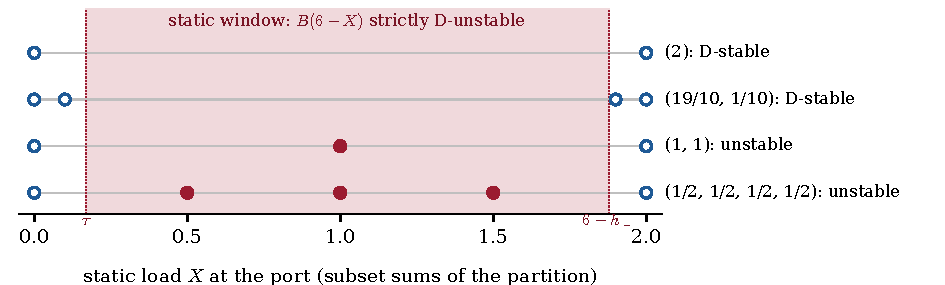
\includegraphics[width=\textwidth]{figures/loading_window.pdf}
\caption{Theorem~\ref{thm:family} for the core $B(6)$ at total load $2$. The
shaded interval is the static window where $B(6-X)$ is strictly D-unstable.
Dots are the subset sums of each partition; a filled dot inside the window
certifies instability (Proposition~\ref{prop:subsetsum}). Partitions without
such a dot are D-stable (Theorem~\ref{thm:family}).}
\label{fig:window}
\end{figure}

\begin{corollary}[Load two on $B(6)$]\label{cor:G2}
Attach a partition $r$ of $G\in(0,2]$ to the port of $B(6)$.
\begin{enumerate}[label=(\roman*)]
\item If $G\le\tau=6-h_+\approx0.1683$, then $A_r$ is D-stable.
\item If $\tau<G<6-h_-\approx1.8787$, then every partition has a strictly
unstable scaling.
\item If $6-h_-\le G\le2$, then $A_r$ is D-stable if and only if its largest
piece satisfies
\[
 \max_jr_j\ \ge\ 6-h_-=\frac{7963+329\sqrt{409}}{7780}\approx1.878742 .
\]
\end{enumerate}
\end{corollary}
\begin{proof}
(i) All subset sums are at most $G\le\tau$. (ii) $G$ itself is a subset sum
in the window. (iii) Let $\ell=\max_jr_j$. If $\ell\ge6-h_-$, the sums
containing the largest piece are at least $6-h_-$. The others are at most
$G-\ell\le2-(6-h_-)=h_--4\approx0.1213<\tau$. So no sum lies in the window. If
$\tau<\ell<6-h_-$, the largest piece is itself in the window. If $\ell\le\tau$,
the partial sums in any order increase in steps at most $\tau$ from $0$ to
$G\ge6-h_-$. The first partial sum exceeding $\tau$ is
then at most $2\tau<6-h_-$, so it lies in the window.
\end{proof}

At total two the verdict thus depends on the split alone, and sharply. The
single site class $(2)$ and the split $(19/10,1/10)$ are D-stable for all
kinetics, as is $(47/25,3/25)$ with its largest piece $1.88$. The split
$(15/8,1/8)$, with largest piece $1.875$, is not: its sum $15/8$ lies in the
window. Neither are $(1,1)$ and its refinement $(\tfrac12,\tfrac12,\tfrac12,
\tfrac12)$. Table~\ref{tab:verdicts} summarizes these verdicts.

\begin{table}[t]
\centering
\caption{Exact verdicts at total load $2$ on $B(6)$.}
\label{tab:verdicts}
\begin{tabular}{@{}llll@{}}\toprule
Partition & Subset sums in $(0,2)$ & Verdict & Reason\\\midrule
$(2)$ & none & D-stable & Theorem~\ref{thm:family}\\
$(19/10,1/10)$ & $1/10,\ 19/10$ & D-stable & Theorem~\ref{thm:family}\\
$(47/25,3/25)$ & $3/25,\ 47/25$ & D-stable & Theorem~\ref{thm:family}\\
$(15/8,1/8)$ & $1/8,\ 15/8$ & strictly unstable scaling & $15/8$ in window\\
$(1,1)$ & $1$ & strictly unstable scaling & explicit witness below\\
$(\tfrac12,\tfrac12,\tfrac12,\tfrac12)$ & $\tfrac12,1,\tfrac32$ & strictly unstable scaling & refinement of $(1,1)$\\
\bottomrule\end{tabular}
\end{table}

\paragraph{An explicit moderate-spread witness.}
Proposition~\ref{prop:subsetsum} gives existence only; its rates are extreme.
For $(1,1)$ an explicit rational witness is
\[
 D=\diag\bigl(\tfrac{617}{1000},\tfrac{617}{1000},\tfrac{617}{1000},35,\tfrac{158}{5},\tfrac{4}{125}\bigr)
\]
(three inner core rates, the port rate, and the two attachment rates). The
characteristic polynomial of $DA_{(1,1)}$ has coefficients, in descending order,
\begin{gather*}
 1,\quad \frac{243483}{1000},\quad\frac{29034069433}{5000000},\quad
 \frac{63896127507669}{12500000000},\\
 \frac{36179911928121089}{6250000000000},\quad
 \frac{76473766154601901}{15625000000000},\quad
 \frac{3507069622203}{3906250000000}.
\end{gather*}
Its exact Routh first column has signs $+,+,+,+,-,+,+$ with no zero pivot, so
there are exactly two roots with positive real part, numerically
$0.0021\pm1.0002i$. The spread is $\kappa(D)=4375/4=1093.75$. The mechanism is
visible in the rates: one attachment is about a thousand times faster than the
other. The fast one acts as a static load of about $1$, which lies in the
middle of the window, while the slow one supplies the lag.
Figure~\ref{fig:envelopes} shows the corresponding contact in the planar
picture. By Corollary~\ref{cor:merge}, equal rates within the halves give the
same two unstable roots for $(\tfrac12,\tfrac12,\tfrac12,\tfrac12)$, plus two
extra eigenvalues $-158/5$ and $-4/125$.

\begin{figure}[t]
\centering
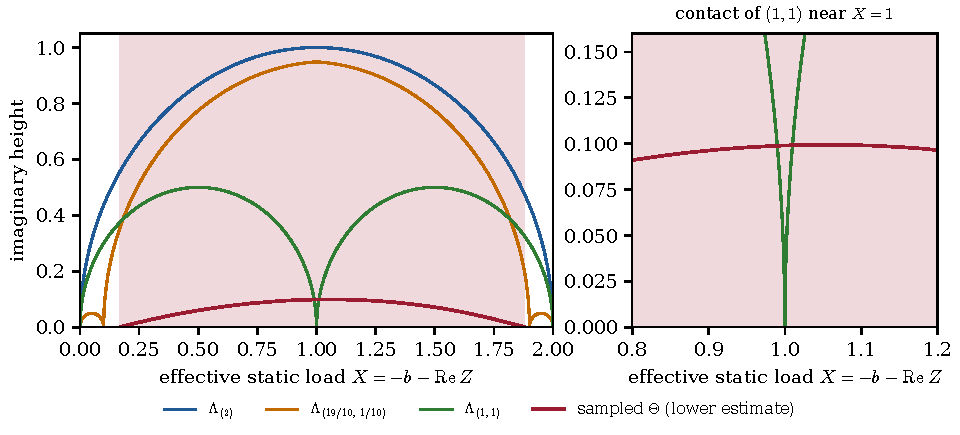
\includegraphics[width=\textwidth]{figures/protection_envelopes.pdf}
\caption{Planar picture for $B(6)$ at total load $2$. Curves show the
protection envelopes $\Env_r$ of Lemma~\ref{lem:image} for the partitions
$(2)$, $(19/10,1/10)$ and $(1,1)$, and a sampled lower estimate of the core
envelope $\Core$ of \eqref{eq:coreenv}, obtained from $6\times10^5$ inner
rate triples. The sampled $\Core$ is positive on the static window, shaded,
and nowhere else, as it must be (Section~\ref{sec:extensions}). The $(1,1)$ envelope vanishes at the subset sum $X=1$, where the core
envelope is about $0.1$ (right panel), so a contact exists. The sampled curve
is an illustration only; the verdicts are proved by exact certificates.}
\label{fig:envelopes}
\end{figure}

% =========================================================================
\section{Several ports, reciprocal modules and hubs}\label{sec:extensions}

\subsection{Several coordinate ports}
Let $\mathcal P$ be a set of distinct coordinates. At each $p\in\mathcal P$
attach a partition with total $G_p>0$. Put $B_X=B+\sum_{p}X_pe_pe_p^{T}$ and
let $\mathcal U=\prod_{p}(0,G_p)$ be the open box.

\begin{theorem}[Open-box criterion]\label{thm:box}
Let $B$ be D-stable. Every choice of finite positive partitions with totals
$(G_p)$ is D-stable if and only if no $B_X$ with $X\in\mathcal U$ has a strictly
unstable positive scaling and $\det B_G\ne0$.
\end{theorem}
\begin{proof}
\emph{No strict growth on $\mathcal U$ implies D-stability on $\mathcal U$.}
Fix positive inverse rates $Q$ and consider $f(X)=\det(iQ-B_X)$. Each $X_k$
enters only the $(k,k)$ entry, so $f$ is affine in each coordinate separately:
$f=f|_{X_k=0}+X_k\,\partial_kf$, and $\partial_kf=-c_k$ is minus the $(k,k)$
cofactor, which does not involve $X_k$. Suppose $f(X^0)=0$ with
$X^0\in\mathcal U$. If some $\partial_kf(X^0)\ne0$, the argument of
Lemma~\ref{lem:marginal} at port $k$ produces strict growth at loads that differ
from $X^0$ only in the $k$-th coordinate by an arbitrarily small amount. These
loads lie in $\mathcal U$, a contradiction. Hence all partials vanish at every
zero in $\mathcal U$. The restriction of $f$ to a coordinate line through $X^0$
is affine with value and slope zero, so $f$ vanishes on the whole segment of
that line in $\mathcal U$. Each point reached is again a zero with vanishing
partials. Moving one coordinate at a time reaches every point of the box, so
$f\equiv0$ on $\mathcal U$, and $f$ is identically zero as a polynomial. Then
$f(0)=\det(iQ-B)=0$, contradicting D-stability of $B$. At zero frequency,
$f_0(X)=\det(-B_X)\ge0$ on $\mathcal U$: a negative value would give a positive
real eigenvalue of $Q^{-1}B_X$. A nonnegative affine function of one coordinate
that vanishes at an interior point has zero slope, and the same propagation
gives $\det(-B)=0$, a contradiction.

\emph{Sufficiency.} Apply Lemma~\ref{lem:absorb} independently at each port.
A nonzero closed-right-half-plane eigenvalue becomes an eigenvalue of a
positive scaling of some $B_X$, $X\in\mathcal U$, which is excluded. Zero is
excluded by $\det(-A)=\det(-B_G)\ne0$.

\emph{Necessity.} If some $B_X$, $X\in\mathcal U$, has strict growth, apply
Lemma~\ref{lem:finite} at every port, subtracting the respective shifts from
the port inverse rates. This gives sufficiently fine partitions that realize
the same eigenvalue. If $\det B_G=0$, every choice is singular.
\end{proof}

No stability assumption on the faces of the box is needed. Strict growth on a
face persists at nearby interior points, because strict growth is an open
condition.

\subsection{Reciprocal relaxation modules}

\begin{corollary}[Reciprocal relaxation safety]\label{cor:relax}
Let a module with state $\zeta$ obey $\dot\zeta=D_\zeta(M\zeta+wx_p)$ and return
$\alpha w^{T}\zeta$ to the port, where $M=M^{T}$ is negative definite and
$\alpha>0$. For every positive $D_\zeta$ the module acts on the port as a
partition with total $G=\alpha w^{T}(-M)^{-1}w$, which is independent of
$D_\zeta$. Theorem~\ref{thm:safety} and part (i) of
Theorem~\ref{thm:threshold} therefore hold with this total, for any number of
such modules at one port. The sufficiency part of Theorem~\ref{thm:box} holds for modules at several
ports. The necessity part does not carry over, because it needs arbitrarily
fine partitions.
\end{corollary}
\begin{proof}
Let $S=D_\zeta^{1/2}MD_\zeta^{1/2}$, which is negative definite, and
$u=D_\zeta^{1/2}w$. Eliminating the module at a candidate eigenvalue $\lambda$
gives the port term
$H(\lambda)=\alpha w^{T}(\lambda I-D_\zeta M)^{-1}D_\zeta w=\alpha u^{T}(\lambda I-S)^{-1}u$.
By the spectral theorem,
\[
 H(\lambda)=\sum_\ell\frac{a_\ell}{\lambda+\lambda_\ell}=\sum_\ell\frac{g_\ell}{1+\lambda/\lambda_\ell},
 \qquad a_\ell\ge0,\ \lambda_\ell>0,\ g_\ell=a_\ell/\lambda_\ell,
\]
with $\sum_\ell g_\ell=H(0)=\alpha w^{T}(-M)^{-1}w$. This is exactly
$L_r(\lambda)$ for the partition $(g_\ell)$ with inverse rates $1/\lambda_\ell$;
zero residues are omitted. Its poles lie in the open left half-plane, so the
elimination is valid in the closed right half-plane, and the proofs of
Theorems~\ref{thm:safety} and~\ref{thm:box} apply verbatim. The zero-frequency
identity $\det(-A)=\det(-M)\det(-B_G)$ with $\det(-M)>0$ handles
$\lambda=0$.
\end{proof}

More generally, if $H_0$ is a positive diagonal symmetrizer, meaning that
$H_0M$ is symmetric negative definite, the reciprocal return is
$\alpha w^{T}H_0\zeta$. The corollary is a \emph{safety} statement. Its converse
would require tuning the modal loads $g_\ell$ independently, which a fixed
indivisible module does not allow.

\subsection{A hub joining D-stable modules}
The planar test has a natural generalization. Let a scalar hub with
self-coefficient $b$ be joined to modules $M_j$ with inputs $w_j$ (from the
hub) and returns $c_j^{T}$ (to the hub), and no direct coupling between
modules. Assume every $M_j$ is D-stable, and put
\[
 V_j=\{c_j^{T}(iQ_j-M_j)^{-1}w_j:\ Q_j>0\text{ diagonal}\},\qquad
 G_j=c_j^{T}(-M_j)^{-1}w_j .
\]

\begin{theorem}[Hub value-set criterion]\label{thm:hub}
The hub-and-module matrix is D-stable if and only if
\[
 -b-\sum_jG_j>0\qquad\text{and}\qquad
 \Bigl(\sum_jV_j\Bigr)\cap\{-b+iq:\ q>0\}=\varnothing .
\]
\end{theorem}
\begin{proof}
Each module pencil $iQ_j-M_j$ is invertible because $M_j$ is D-stable. After
frequency normalization, eliminating the modules turns a contact into
$iq_h-b-\sum_jH_j=0$ with $H_j\in V_j$; a zero hub component would force every
module component to vanish. Since $q_h>0$ is free, contacts are exactly the
points of the Minkowski sum on the stated ray. At zero,
$\det(-A)=\prod_j\det(-M_j)\,(-b-\sum_jG_j)$ with every $\det(-M_j)>0$, so the
first condition is necessary and excludes zero eigenvalues. For a base point,
fix module rates and let the hub rate $d_h$ tend to $0$. One eigenvalue tends
to $0$ and the others to the Hurwitz spectra of the scaled modules. The
determinant comparison of Theorem~\ref{thm:partition} gives the small real
eigenvalue $d_h(b+\sum_jG_j)(1+o(1))<0$. Connectedness of the positive cone
and continuity of eigenvalues conclude.
\end{proof}

Theorem~\ref{thm:partition} is the case of one inner module (the inner block
$C$) together with scalar modules $M=(-1)$, $w=1$, $c=r_j$, whose value sets
are the semicircles $\{r_j/(1+it)\}$. Because the inner block of a D-stable
matrix need not be D-stable, Theorem~\ref{thm:partition} treats singular inner
pencils separately.

\begin{corollary}[Negative-imaginary modules]\label{cor:ni}
If every $V_j$ lies in the closed lower half-plane, then the hub system is
D-stable if and only if $-b-\sum_jG_j>0$. This holds in particular for
reciprocal relaxation modules.
\end{corollary}
\begin{proof}
The ray has positive imaginary part. For reciprocal modules,
$\Imag\sum_\ell g_\ell/(1+i/\lambda_\ell)=-\sum_\ell g_\ell\lambda_\ell^{-1}/(1+\lambda_\ell^{-2})\le0$.
\end{proof}

A stable scalar transfer function with $\Imag H(i\omega)\le0$ for $\omega>0$
is negative imaginary. Corollary~\ref{cor:ni} is thus a D-stability counterpart of
the theorem of Lanzon and Petersen~\cite{lanzon2008,xiong2010}, in which a
suitable DC gain condition decides stability of a negative-imaginary
interconnection. The granularity phenomenon needs the opposite ingredient: a
module, here the core's inner block, whose value set reaches the upper
half-plane at the relevant real part. That happens exactly where $\Core>0$. For
$B(6)$ this is precisely the open static window. Inside it, $B_X$ has strict
growth and $\det(-B_X)>0$. It also has a Hurwitz scaling: with the port rate
$v\to0$ the third Hurwitz determinant tends to $F_0>0$ (proof of
Proposition~\ref{prop:Bh}). So along a path of scalings from a stable one
some eigenvalue crosses the imaginary axis away from zero; singular inner pencils
carry no contacts (proof of Theorem~\ref{thm:partition}). Outside its closure,
$B_X$ is D-stable.

% =========================================================================
\section{Binding sites, decoys and buffers}\label{sec:application}

\paragraph{Dictionary.}
Consider a linearized system $\dot x=DJx$ in which $J$ is the flux Jacobian at
a steady state. $D$ is the positive diagonal matrix of inverse
\emph{capacities}: compartment volumes, buffering capacities or turnover
scales, which are unknown. Let the port species bind to site classes
$j=1,\dots,m$. Class $j$ has linearized binding coefficient $k_j$ (on-rate
times free-site concentration), unbinding rate $u_j$ and degradation
$\delta_j\ge0$ of the bound complex $y_j$:
\[
 \dot x_p\ \ni\ -k_jx_p+u_jy_j,\qquad \dot y_j\ \propto\ k_jx_p-(u_j+\delta_j)y_j .
\]
In the notation of Section~\ref{sec:normalization}, $a_j=u_j$, $c_j=k_j$ and
$h_j=u_j+\delta_j$. The normalized model has core
$B=J_{\mathrm{core}}-\bigl(\sum_jk_j\bigr)e_pe_p^{T}$ and loads
\[
 r_j=\frac{k_ju_j}{u_j+\delta_j},
\]
with free attachment rates $(u_j+\delta_j)$ times the inverse capacity of
$y_j$. A slow site class, whose complexes are effectively frozen, acts as a pure
loss $k_j$ on the port. A fast class equilibrates instantly, and its net
effect on the port diagonal is $-k_j\delta_j/(u_j+\delta_j)$. The static
loading interval therefore runs from the loss-only core $B$ (all classes slow)
to the fast-site Schur complement $B_G$ (all classes fast). With no degradation
the two ends are $J_{\mathrm{core}}-\sum_jk_j\,e_pe_p^{T}$ and
$J_{\mathrm{core}}$ itself.

\paragraph{What the theorems predict.}
Suppose that both ends of the interval are D-stable, so that neither a slow
nor a fast binding environment destabilizes the core. If the interior of the
interval contains static strict growth, then
Theorem~\ref{thm:threshold} and Proposition~\ref{prop:subsetsum} predict that
\emph{heterogeneous} site populations can destabilize the core, while a
single homogeneous class may not. The criterion is
combinatorial: some grouping of the site classes into ``fast'' and ``slow''
must place the effective static damping of the port inside the unstable
window. Only dimensionless comparisons enter: the loads $r_j$ and their
subset sums against the window of the static ray, all in the units of the
core's entries. Merging classes never hurts (Corollary~\ref{cor:merge}).
Bounding the ratio of kinetic time scales raises the threshold when
$\det B_\tau\ne0$ (Proposition~\ref{prop:spread}).

\paragraph{The four-state example as a binding problem.}
Take $J_{\mathrm{core}}=B(4)$ and site classes of total binding coefficient
$2$ with $\delta=0$. The loss-only core is $B(6)$ and the fast limit is
$B(4)$; both are D-stable. By Corollary~\ref{cor:G2}, the system is D-stable
for all capacities and unbinding rates if and only if one site class carries
at least $6-h_-\approx1.8787$ of the total binding coefficient. In that case
the remaining classes, whatever their kinetics, cannot move the port into the
window. With two equal classes the linearization has a growing oscillatory mode.
In the explicit witness the effective rates of the two classes differ by a
factor of about $10^3$; this ratio can be carried by the unbinding rates, by
the capacities of the complexes, or by both. This is an exact linear
interface example, not a calibrated biochemical model.

\paragraph{Scope in applications.}
Buffer- and decoy-induced oscillations, and their suppression, are known in
specific nonlinear models~\cite{falcke2003,gin2006,karapetyan2015,dey2021}. So
is the loading effect of downstream binding~\cite{delvecchio2008,jayanthi2013}.
Adding sites to a nonlinear model generally changes its steady state and hence
the core Jacobian, whereas our comparison holds the linearized core fixed. In
particular, a fixed three-state core, such as a Goodwin-type loop, cannot
exhibit the fixed-total granularity effect (Proposition~\ref{prop:small}).
The theorems quantify over \emph{all} positive rates: they are worst-case,
time-scale-robust statements. In a specific kinetic model some rates may be
linked, and the instability conclusions are then existence statements over a
larger parameter set than the model allows. The conclusions concern linear
spectral growth; no statement about Hopf bifurcations or limit cycles is made.

% =========================================================================
\section{Verification and scope}\label{sec:verification}

\paragraph{Formal verification.}
Theorem~\ref{thm:threshold} is verified end to end in Lean~4~\cite{demoura2021}
with Mathlib~\cite{mathlib2020}, including $0\le\tau\le-B_{pp}$ and the complete
equality case. The exported theorem is \texttt{granularity\_threshold} in the
namespace \texttt{DStabilityCharacterization.Granularity}, in the file
\texttt{proofs/DStabilityCharacterization/Threshold.lean}. It is stated for
arbitrary finite index types of core and attachments, with literal
matrix eigenpairs under every positive diagonal scaling. D-stability is
strict: every eigenvalue of every scaling has negative real part. The
fineness $\varepsilon$ in part~(iii) is quantified before the attachment type
and the partition. The proof formalizes Lemma~\ref{lem:absorb},
Theorem~\ref{thm:safety}, Lemma~\ref{lem:marginal}, Lemma~\ref{lem:finite}(a)
with a uniform tolerance, and Lemma~\ref{lem:taubound}. The spread bound of
Lemma~\ref{lem:finite}(b) is not part of the formal statement. It assumes no spectral-continuation, coverage or
realization premise. The strict build (Lean v4.30.0, warnings as errors)
compiled with $19$ project dependencies. The theorem depends only on the
axioms \texttt{propext}, \texttt{Classical.choice} and \texttt{Quot.sound}. The
verified source has SHA-256
\texttt{2e515988238c2dcb4d8b0143f1aa510ca90c7d1bc90421633a24014a70055520}.

\paragraph{Exact computation.}
Lemma~\ref{lem:edgecert} is an exact computer-assisted certificate. The
script \texttt{check\_paper.py} accompanies the source and replays it in
rational and algebraic arithmetic. The same script checks every printed number:
the identities of Lemmas~\ref{lem:absorb} and~\ref{lem:finite}, the
three-state identities of Section~\ref{sec:small}, the coefficients and
Hurwitz decomposition of Proposition~\ref{prop:Bh}, the constants $h_\pm$,
$\tau$ and $6-h_-$, the verdicts of Table~\ref{tab:verdicts}, the witness
polynomial and its Routh signs, and the refinement identity. It also checks
the Lean receipt and its hashes. A few floating-point sanity checks are
labelled as such.

\paragraph{Conventional proofs.}
All other results carry complete conventional proofs here and are not claimed as formally verified: Lemma~\ref{lem:finite}(b),
Proposition~\ref{prop:spread}, Sections~\ref{sec:planar}, \ref{sec:subsets}
and~\ref{sec:small}, Theorem~\ref{thm:family}, Corollary~\ref{cor:G2}, and
Section~\ref{sec:extensions}. Proposition~\ref{prop:Bh} is conventional
reasoning on top of polynomial identities (the coefficients $c_i$ and the
decomposition $\Delta_3=\sum_jF_jv^j$) that are checked by exact computation,
as is the witness for $(1,1)$.

\paragraph{Scope.}
The threshold $\tau$ and the envelope $\Core$ are reductions, not algorithms.
Deciding D-stability of $B_X$ in general, and computing $\Core$ for large
cores, remain as hard as the underlying static problem. The coordinate
structure of the interface is essential: the absorbed lag
$\lambda\alpha\,ee^{T}$ is a legitimate change of the port's rate only because
$ee^{T}$ is diagonal. For a non-coordinate interface $uv^{T}$ the reduction
fails.

% =========================================================================
\section{Open problems}\label{sec:open}

\begin{enumerate}[leftmargin=1.6em]
\item \emph{Computing the core envelope.} Characterize $\Core$ for small inner
blocks, and decide when it is attained at equal inner rates, as it
empirically is for $B(6)$. Sum-of-squares or P{\'o}lya certificates for the disk
conditions of Corollary~\ref{cor:disk} give sufficient tests, and scaled
small-gain relaxations give conservative bounds. An exact efficient method is
not expected in general.
\item \emph{When is the subset-sum test exact?} Characterize the cores for
which D-stable corners imply D-stable edges, as in
Lemma~\ref{lem:edgecert}.
\item \emph{Non-coordinate interfaces.} Find the smallest example in which
phase, rather than static load, sets the threshold.
\item \emph{The time-scale-limited threshold.} Compute $\tau_\kappa$ of
Proposition~\ref{prop:spread}, and its asymptotics as $\kappa\to\infty$, for
the family of Section~\ref{sec:family}. Relatedly, determine the minimal
spread of an unstable scaling as a partition approaches the boundary of the
window.
\item \emph{Random heterogeneity.} For random loads and log-uniform time
scales, find the probability of instability as the number of pieces grows.
\item \emph{Networks of modules.} Extend the hub criterion to trees of modules
glued at single coordinates, via a recursion of planar value sets.
\item \emph{Nonlinear onset.} Decide whether the crossing of the window by a
subset sum produces a supercritical Hopf bifurcation in a realized kinetic
model.
\end{enumerate}

\section*{Data and code availability}
The Lean sources, the verification receipt, \texttt{check\_paper.py} and
\texttt{make\_figures.py} are part of the accompanying repository. The
manifest \texttt{ARTIFACT\_MANIFEST.json} lists their SHA-256 hashes.

\bibliographystyle{plainurl}
\bibliography{refs}

\end{document}
